\chapter{Motivating Scenario}
\label{chap:motivatingScenario}
In order to help in understanding the concepts of organizational modeling, a motivating scenario has been taken and explained through the modeling notations mentioned in Section \ref{sec:resourcecentricorganizationalmodeling} of Chapter \ref{chap:fundamentals}. This scenario also helps in validating the developed web-based modeling tool in the following Chapter \ref{chap:casestudy}. The motivating scenario has been chosen based on the collected real life scenarios provided in another thesis work \cite{Sierr2015}. The motivating scenario was taken from the context of manufacturing sector. 

In this chapter, the first section provides a brief introduction about the motivating scenario. The last section provides an abstract overview about the organizational modeling elements discussed in motivating scenario. This abstract concepts are explained in a concrete way in the following Chapter \ref{chap:casestudy}.

%%%%%%%%%%%%%%%%%%%%%%%%%%%%%%%%%%%%%%%%%%%%%%%%%%%%%%%%%%%%%%%%%%%%%%%%%
\section{Intention-oriented Organizational Modeling Example}
\label{sec:scenario}
%%%%%%%%%%%%%%%%%%%%%%%%%%%%%%%%%%%%%%%%%%%%%%%%%%%%%%%%%%%%%%%%%%%%%%%%%
 The concept of resource centric organizational modeling can be explained with the following scenario taken from a manufacturing organization. Consider a budding manufacturing company which designs, develops, manufactures and sells personal computers, tablets and laptops. The CEO's main intention of the quarter is \textit{to increase the revenue and number of unit sales}. The initial context describes the situation before starting the execution of intention. The initial context also provides statement that motivates to start the process. The final context describes the situation that is achieved once the intention executed successfully. Intentions connect initial context definitions with final context definitions \cite{Sungur2014a}. There are also low level intentions other than the main intention which helps in achieving main intention in a measurable form. Intentions contain strategies implementations through achieving strategies which are plans of action designed to meet a specific intention. 
 
  \begin{figure}
  	\centering
  	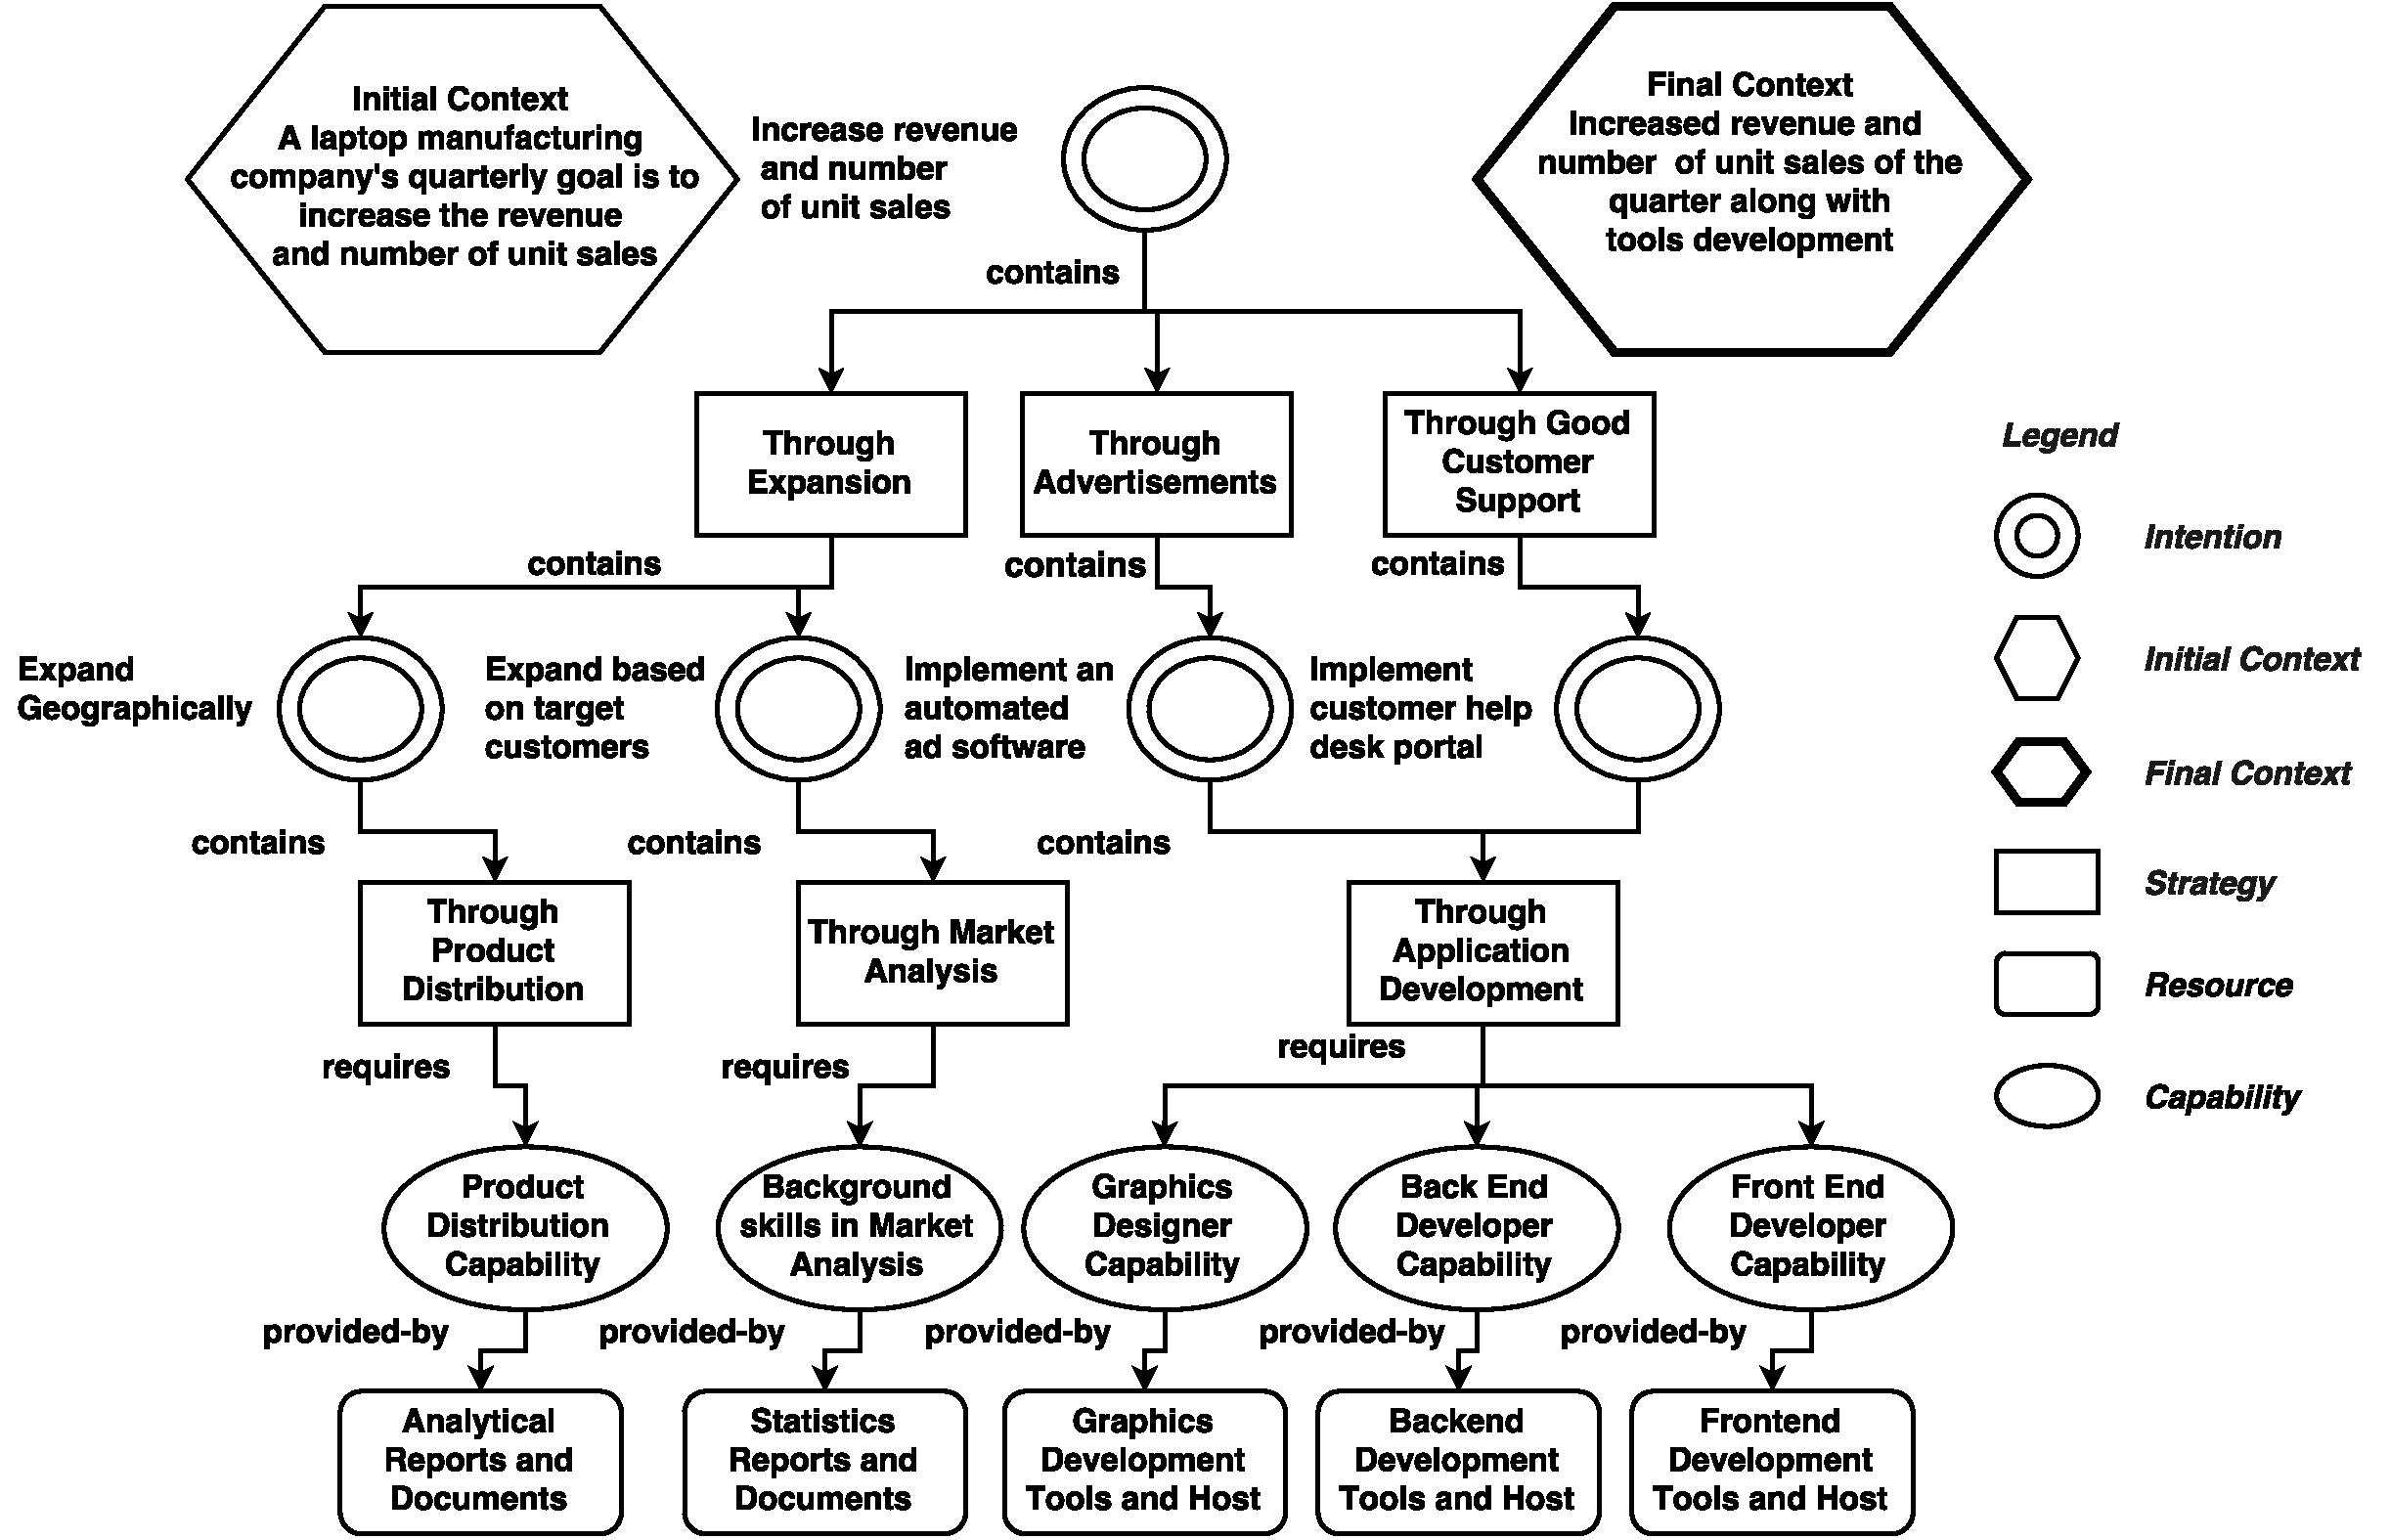
\includegraphics[width=\textwidth,angle=0]{MotivatingScenario.pdf}
  	\caption{Motivating Scenario}
  	\label{fig:motivatingscenario}
  \end{figure}
  
The Figure \ref{fig:motivatingscenario} provides the details of organizational intentions, strategies, capabilities and resources. There can be multiple strategies followed to achieve a main intention. The main intention can be achieved by following all of the below mentioned strategies which requires resources with matching capabilities associated with these strategies. 
 
 \begin{enumerate}
 	\item Increasing the revenue through expanding the market sales. 
 	\item Through increasing the advertisement which helps customer to know about the product.
 	\item Improving the existing customer help desk portal, as it helps to maintain good customer relationship.
 \end{enumerate}
 
%%%%%%%%%%%%%%%%%%%%%%%%%%%%%%%%%%%%%%%%%%%%%%%%%%%%%%%%%%%%%%%%%%%%%%%%%
\section{Organizational Modeling Elements}
\label{sec:entities}
%%%%%%%%%%%%%%%%%%%%%%%%%%%%%%%%%%%%%%%%%%%%%%%%%%%%%%%%%%%%%%%%%%%%%%%%%
It is important to explain each of the organizational modeling element using an example as it helps in understanding the requirements of intention-oriented organizational modeling discussed in the Section \ref{sec:requirementssupoorting} of following Chapter \ref{chap:analysis}. Before we proceed with detailed description of each modeling elements we provide an example scenario to know the dynamic nature of organizational modeling. For example, in our above mentioned motivating scenario in Section \ref{sec:scenario} one of the intention is to \textit{expand sales geographically}. Before executing this intention, few ground works like collection of laptop usage statistics such as average buying capacity of the consumers, average computer knowledge of the people in new geographic location has to be done. Thus the execution of main intention i.e \textit{increase revenue and number of unit sales}, requires collaboration of people with different skills and expertise. For example, resources with skills to collect and study statistics are required. If in case none of the organizational resources provide required capability then the organization can get it served from external resources or further modularize the intention so that it can be provided by internal resources itself. This makes to emerge new intentions dynamically. The team working towards achievement of main intention should also be ready to accommodate new resources with new capabilities and skills. For example, there is a software development team, which work towards achievement of the intention \textit{improve help desk portal}, i.e., this team develops software that automatically attends and records user queries. Suppose, if there arise a new requirement of \textit{supporting help desk through mobile applications} as well then the system should accommodate new resource with \textit{mobile application developer} capability. 

%%%%%%%%%%%%%%%%%%%%%%%%%%%%%%%%%%%%%%%%%%%%%%%%%%%%%%%%%%%%%%%%%%%%%%%%%
\subsection{Contexts} 
\label{sec:contexts}
%%%%%%%%%%%%%%%%%%%%%%%%%%%%%%%%%%%%%%%%%%%%%%%%%%%%%%%%%%%%%%%%%%%%%%%%%
The execution of manufacturing processes such as the one provided in Figure \ref{fig:motivatingscenario} are not similar to execution of typical business processes. This is because, the execution of manufacturing processes mostly depends on the information collected from the real world, i.e., the execution context \cite{Sungur2016}. A context definition provides mechanism to act adaptively based on the current situation. This is achieved in the production environment by describing each process with a specific context definition \cite{Sungur2016}. For example, in our motivating scenario the initial context provides details about status before achievement of the main intention i.e it specifies the situation of the organization which triggers the execution of main-intention. The initial context \textit{quarterly goal of increasing the revenue and number of unit sales}, helps to decide the main intention and its related low level associates. On successful achievement of main-intention the organization reaches it desired final context of \textit{increased revenue and number of unit sales}. Along with successful reaching of the final context, this also provides tools such as web-based help desk portals, automated ad software etc., that are developed as part of this execution. When the final context definition has been reached the process completion starts. This process final state can be stored \cite{Sungur2015b} and same set of resources can be re-used in future executions with similar contexts and intentions.
 
%%%%%%%%%%%%%%%%%%%%%%%%%%%%%%%%%%%%%%%%%%%%%%%%%%%%%%%%%%%%%%%%%%%%%%%%%
\subsection{Intentions} 
\label{sec:intentions}
%%%%%%%%%%%%%%%%%%%%%%%%%%%%%%%%%%%%%%%%%%%%%%%%%%%%%%%%%%%%%%%%%%%%%%%%%
Intentions are defined hierarchically, in our approach intentions are located in top level of the hierarchy, which are refined until concrete lower level of the hierarchy is reached. In this thesis context, intentions are not associated with capabilities directly, instead intentions are associated with strategies which are then associated with capabilities. For example, in our motivating scenario the main intention is to increase revenue and number of unit sales which also has sub-intention of \textit{improving the customer help desk portal} and strategies such as 1. through expanding sales and 2. through advertisements. The relation between strategies and intentions are denoted by the term \textit{contains} in Figure \ref{fig:motivatingscenario} as strategies are methods through which intentions can be achieved. There can be situation where an intention can be related to another intention. For example, consider a situation in our motivating scenario where customer help desk team not willing to give up the systems they are working for a long time even if it is a better solution for organization as whole. This can also happen in every organizations, where a real life scenario has been provided in the thesis work \cite{Sierr2015} and also it has been suggested that such intentions are called contradicting intentions and it has to be handled in some way by the modeling approach. 

%%%%%%%%%%%%%%%%%%%%%%%%%%%%%%%%%%%%%%%%%%%%%%%%%%%%%%%%%%%%%%%%%%%%%%%%%
\subsection{Strategies} 
\label{sec:strategies}
%%%%%%%%%%%%%%%%%%%%%%%%%%%%%%%%%%%%%%%%%%%%%%%%%%%%%%%%%%%%%%%%%%%%%%%%%
Strategies are used to identify the most appropriate method of utilizing capabilities through which an intention can be achieved. Strategies are associated with both intentions and capabilities. Each strategy needs certain capability to successfully execute an intention. So we need to associate strategy with a capability that has matching resource. Resources are the potential holder of the capability i.e., to satisfy a capability we need resources. Capability and its associated resources are also shown in the Figure \ref{fig:motivatingscenario}. In our motivating scenario, the main intention can be achieved through two strategies \textit{through expansion} and \textit{through advertisements}. These two strategy further contains intentions such as \textit{expand geographically}, \textit{expand based on target customers} and \textit{implement an automated ad software}. Since strategies contain intentions they are related through the term \textit{contains} in the Figure \ref{fig:motivatingscenario}. As mentioned earlier, informal process models are realized through strategies. This is achieved through strategy containing capabilities and resources. For example, consider a small part in our motivating scenario of achieving an intention expand geographically through strategy product distribution. To achieve this intention through a specified strategy we need resources with product distribution capability. This results in informal process as a strategy that has capabilities, resources that are created out of capabilities and an intention of that specific strategy.

%%%%%%%%%%%%%%%%%%%%%%%%%%%%%%%%%%%%%%%%%%%%%%%%%%%%%%%%%%%%%%%%%%%%%%%%%
\subsection{Capabilities}
\label{sec:capabilities}
%%%%%%%%%%%%%%%%%%%%%%%%%%%%%%%%%%%%%%%%%%%%%%%%%%%%%%%%%%%%%%%%%%%%%%%%%
Resources tend to posses certain capabilities that allow them to do something that they want or need to do something. Each organizational capability must be provided by a resource in the organization. Resource models are optional \cite{Sungur2015b} to make precise definitions of resources needed. In our context, capabilities that are associated with resources are called as \textit{functional capabilities}. The type of capability that contains functional capabilities are called as \textit{cross functional capabilities}. Strategies are associated with cross functional capabilities, which contains functional capabilities out of which resources are created. In our motivating scenario to achieve the main intention, we need several capabilities such as product distribution capability, graphics designer capability etc. Thus in the Figure \ref{fig:motivatingscenario}, strategies and associated capabilities are related through the term \textit{requires}. 

%%%%%%%%%%%%%%%%%%%%%%%%%%%%%%%%%%%%%%%%%%%%%%%%%%%%%%%%%%%%%%%%%%%%%%%%%
\subsection{Resources} 
\label{sec:resources}
%%%%%%%%%%%%%%%%%%%%%%%%%%%%%%%%%%%%%%%%%%%%%%%%%%%%%%%%%%%%%%%%%%%%%%%%%
Each resources has different types of relationship with other resources based on how they communicate with other resources \cite{Sungur2015}. For example in our motivating scenario described in Section \ref{sec:scenario} has an intention to \textit{improve customer help desk portal}. This intention can be achieved by providing skills improvement training to the employees or by recruiting newly skilled employee. Here the manager has permissions to decide whether to improve skills of existing employee or recruit new employee. But the team lead has restricted permission like what type of skills are required for the project based on decision of manager. 
